\documentclass[]{article}
\usepackage[letterpaper, margin = 1in, footskip = 0.25in]{geometry}
\usepackage{amsmath,amssymb,setspace,mathabx}
\usepackage{graphicx}
\usepackage{lscape}
\usepackage{verbatim}
\usepackage{rotating}
\usepackage{framed}
\usepackage{booktabs}
\usepackage{longtable}
\usepackage{array}
\usepackage{multirow}
\usepackage[table]{xcolor}
\usepackage{wrapfig}
\usepackage{float}
\usepackage{colortbl}
\usepackage{pdflscape}
\usepackage{tabu}
\usepackage{threeparttable}
\usepackage{threeparttablex}
\usepackage[normalem]{ulem}
\usepackage{makecell}
\usepackage{caption}
\usepackage{pdflscape}
\newcommand{\blandscape}{\begin{landscape}}
\newcommand{\elandscape}{\end{landscape}}



\doublespacing

\font\myfont=cmr12 at 15pt

\providecommand{\tightlist}{%
  \setlength{\itemsep}{0pt}\setlength{\parskip}{0pt}}

% Redefine \includegraphics so that, unless explicit options are
% given, the image width will not exceed the width of the page.
% Images get their normal width if they fit onto the page, but
% are scaled down if they would overflow the margins.
\makeatletter
\def\ScaleIfNeeded{%
  \ifdim\Gin@nat@width>\linewidth
    \linewidth
  \else
    \Gin@nat@width
  \fi
}
\makeatother

\let\Oldincludegraphics\includegraphics
{%
 \catcode`\@=11\relax%
 \gdef\includegraphics{\@ifnextchar[{\Oldincludegraphics}{\Oldincludegraphics[width=\ScaleIfNeeded]}}%
}%

\setcounter{secnumdepth}{5}


\ifxetex
  \usepackage[setpagesize=false, % page size defined by xetex
              unicode=false, % unicode breaks when used with xetex
              xetex]{hyperref}
\else
  \usepackage[unicode=true]{hyperref}
\fi
\hypersetup{breaklinks=true,
            bookmarks=true,
            pdfauthor={Sean P. Cox, Samuel D. N. Johnson, Stephen P. Rossi},
            pdftitle={Two classes of multi-model candidate management procedures for Atlantic bluefin tuna.},
            colorlinks=true,
            citecolor=blue,
            urlcolor=blue,
            linkcolor=magenta,
            pdfborder={0 0 0}}
\urlstyle{same}  % don't use monospace font for urls

\title{Two classes of multi-model candidate management procedures for Atlantic bluefin tuna.}
\author{Sean P. Cox, Samuel D. N. Johnson, Stephen P. Rossi}
\date{}
\usepackage{booktabs}
\usepackage{longtable}
\usepackage{array}
\usepackage{multirow}
\usepackage[table]{xcolor}
\usepackage{wrapfig}
\usepackage{float}
\usepackage{colortbl}
\usepackage{pdflscape}
\usepackage{tabu}
\usepackage{threeparttable}
\usepackage{threeparttablex}
\usepackage[normalem]{ulem}
\usepackage{makecell}
\usepackage{caption}
\usepackage{pdflscape}

% Bibliography stuff




\begin{document}
% Frontmatter

% Start line numbers

% Title Page
\begin{titlepage}

\begin{flushleft}


\noindent
\textbf{Two classes of multi-model candidate management procedures for Atlantic bluefin tuna.}\\[0.2in]

{Sean P. Cox, Samuel D. N. Johnson, Stephen P. Rossi, }

\vspace{0.2in}

\vspace{0.2in}

\textbf{Abstract} \\
We developed two classes of management procedures for Atlantic bluefin tuna based on multi-model inference. The basis of the procedures were estimation methods tuned to five operating models from the reference OM grid. For the empirical class, we used OM catchability and a stationary stock mixing distribution to estimate area biomass from the larval indices. For model-based class of MPs, we tuned 5 delay difference assessment models to each of the 5 operating models, matching stock recruit steepness and biomass for the recent historical period from 1965 - 2016. At each time step, estimates of current (empirical) or projected (model-based) biomass were generated from approved management indices. These estimates were used in harvest control rules to generate area-specific TACs, and the five TACs were averaged to produce harvest advice for the East and West area. Multiple MPs were then defined based on varying precautionary TAC caps, maximum target harvest rates, and HCR control points. We found that MPs with lower caps, lower maximum harvest rates and control points avoided overfishing on the reference grid more often. We also found that the subset of OMs that our AMs were tuned to managed to capture the uncertainty well. \\[0.2in]
\end{flushleft}

\today

\end{titlepage}

\setcounter{page}{2}


% End Title Page



\newpage

{
\hypersetup{linkcolor=black}
\setcounter{tocdepth}{2}
\tableofcontents
}
\hypertarget{introduction}{%
\section{Introduction}\label{introduction}}

The International Commission for the Conservation of Atlantic
Tunas (ICCAT) is currently conducting a management strategy evaluation (MSE)
for Atlantic bluefin tuna (ref ICCAT 2019). The technical core
of an MSE is closed loop simulation testing of candidate managment
procedures (CMPs) that provide harvest advice in the presence
of uncertainty. Uncertainty is captured by a set of operating models,
which represent a plausible range of states for the
management system.

The operating models for Atlantic bluefin tuna are based on different
hypotheses (fits) of a multi-stock, multi-area, age- and length-structured
model known as the Modifiable Multi-stock Model (M3), with 4 fishing
seasons per year, that allow for mixing of fish from both stocks in each area in a given
season (\textbf{REF TSD}). Given the inherent complexity of such
a model, it is impossible to use the same structure within a management
procedure, as management procedures must be able to be tested within
simulations in a timely manner. Therefore, management procedures must
be designed that are of lower levels of complexity than the operating model.

In this paper, we develop and test two classes of CMPs that use multi-model inference
to provide harvest advice in the MSE framework. The first class is
based on an empirical index-based method of estimating spawning stock
biomass, and the second replaces the empirical method with a multi-stock
state-space delay difference stock assessment model. Both classess are
made up of five biomass estimation and harvest control rules that are
tuned to one of five reference grid operating models. Catch advice from each
sub-procedure is then combined to produce area-specific TACs.

\hypertarget{methods}{%
\section{Methods}\label{methods}}

Our candidate management procedures were based on multi-model inference
{[}@rossi2019inferring{]}, combining estimates of biomass and associated catch
advice from sub-procedures tuned to a subset of the reference grid of
multi-stock operating models. This multi-model formulation allowed us to
capture the biological uncertainty represented by the reference grid
of operating models.

We defined two classes of MP: empirical and model based. The empirical MPs
scale larval indices by OM estimates of catchability, while the
model-based MPs fit state space delay difference assessment model
to management indices.

\hypertarget{choice-of-operating-models}{%
\subsection{Choice of operating models}\label{choice-of-operating-models}}

We chose a tuning subset of five reference grid operating models,
namely OMs 1, 2, 4, 7, and 11, to tune our estimation procedures.
These five OMs were chosen to span the three main axes
of operating model uncertainties (stock-recruit steepness, natural
mortality/maturity, and stock mixing), as well as the range of spawning
stock biomass scales and dynamics (Figure 1).

\hypertarget{empirical-estimation-procedure}{%
\subsection{Empirical Estimation Procedure}\label{empirical-estimation-procedure}}

The empirical estimation procedure used a simple moving average of
the two spawning stock larvel survey indices. For each time step \(t\),
and stock \(s \in \{GOM, MED\}\) the current average larvel index is
calculated as
\begin{align}
\bar{I}_{s,t} & = \frac{\sum_{t'= t-3}^{t} I_{s,t'}}{4}, 
\end{align}
where \(I_{s,t}\) is the larval index for stock \(s\) at time \(t\). We then
scaled the smoothed survey indices to multiple biomass estimates, one
for every operating model in the tuning subset, by using the appropriate
larval survey catchability parameter, e.g
\begin{equation}
\hat{B}_{s,t,k} = \frac{\bar{I}_{s,t}}{q_{s,k}},
\end{equation}
where \(q_{s,k}\) is the stock larval index catchability parameter from
the tuning operating model \(k \in \{1,2,4,7,11\}\).

Spawning stock biomass was then translated to area biomass using an
assumed constant distribution of biomass for stock mixing
\begin{equation}
P = (p_{s,a}) =  \left( \begin{array}{cc}
                .898 & .102 \\
                .1 & .9
            \end{array}
    \right),                    
\end{equation}
found by averaging the proportion of stock biomass in each area
over the historical period in the tuning set of OMs. The rows
of matrix \(P\) are indexed by spawning stocks \(\{MED, GOM\}\), and the
columns are indexed by management area \(\{ E, W\}\). This generates
an area specific biomass
\begin{equation}
B_a = \sum_{s} p_{s,a} B_s,
\end{equation}
where \(s \in \{MED, GOM\}\), \(a \in \{E, W\}\).

\hypertarget{delay-difference-model}{%
\subsection{Delay Difference Model}\label{delay-difference-model}}

For the model-based class of procedures, the simple index scaling
method of the empirical procedure is replaced by a state-space
multi-stock delay difference assessment model. The two spawning
stocks are assumed to be distinct spawning stocks for the larval
surveys, but are mixed using the distribution \(P\) for
the other management indices and the observed catches.

\hypertarget{equilibiria}{%
\subsubsection{Equilibiria}\label{equilibiria}}

Because there is no mixing of spawners, each stock has the simple Delay
Difference equilibrium states, which can be expressed as a function
of long-term fishing mortality \(f = F_s\). The equations for equilibria
in Table 1 were used to initialise the model at a fished equilibrium
in 1965, as well as estimate biological reference points for use in
the harvest control rules.

\hypertarget{biomass-time-series-reconstruction}{%
\subsubsection{Biomass time series reconstruction}\label{biomass-time-series-reconstruction}}

Each assessment model was initialised in a fished state in 1965. To do so,
we estimated an initial fishing mortality rate \(F_(s,0)\), and assumed
that the stock was at the fished equilibrium defined in Table 1. Other free
parameters were unfished biomass \(B_{s,0}\), catchability \(q_g\) and
observation error uncertainty \(\tau_g\) for biomass and abundance indices,
and recruitment process error deviations \(\omega_{s,t}\) for
\(t \in 1966,..., 2014\) (Table 2).

We assumed the that proportion \(p_{s,a}\) of
stock\textasciitilde{}\(s \in \{MED,GOM\}\) in area\textasciitilde{}\(a \in \{E,W\}\) was
constant, allowing the fluctuations in stock biomass to
account for the mixing dynamics. We also assumed that the stocks
were homogeneously mixed in each area, so that total stock specific
catch was the sum of the area specific catches, split according
to the proportion to the stock biomass in each area (eqn ref).

We used a numerical Newton-Rhapson method to solve for instantaneous
fishing mortality at all time steps \(t \geq 1\), which were used in
the survival calculation to progress numbers and biomass to the
next time step.

We modeled recruitment process errors as a simple random
walk, rather than indepent deviations from the stock recruit curve.
We chose a random walk as it was more able to capture dynamic
recruitment regimes. Furthermore, random walks would also make
projected recruitments, which are an important component of
projected biomass in a delay difference formulation, less
likely to be average, and more like the estimated
recruitment in the last year of the assessment period.

Because this is a model-based MP and the time-series of approved
management indices are rather short, we included two additional indices.
These indices were the M3 model yearly spawning stock biomass estimates
for the East and West stocks. These biomass time series were assumed to be
observed with catchability \(q = 1\) and an observation error
CV of \(5 \%\). This allowed our AMs to estimate catchability for the
approved indices and scale them appropriately to the spawning stock biomass
from the associated operating model, which was required for extending the
fit to the approved indices in the projections, as well as making sensible
estimates of biological parameters despite the complexity mismatch between
the operating model and the assesment models.

\hypertarget{reference-points}{%
\subsubsection{Reference Points}\label{reference-points}}

Reference points for each stock were estimated from the equilibrium
values in (Table 1). The optimal fishing mortality rate \(F_{MSY}\)
was found by numerically solving for the stationary point of the yield
curve, and was in turn used to estimate the optimal equilibrium
biomass \(B_{MSY}\) associated with that mortality rate.

We estimated area based reference points for use in harvest control
rules, which were the stock-area biomass weighted averages of
the stock-specific reference points, i.e.
\begin{align}
B_{MSY,a} & = \sum_{s} \frac{B_{s,a}}{B_a} B_{MSY,s}, \\
F_{MSY,a} & = \sum_{s} \frac{B_{s,a}}{B_a} F_{MSY,s},
\end{align}
where \(B_{s,a} = p_{s,a} B_s\).

\hypertarget{harvest-control-rules}{%
\subsection{Harvest Control Rules}\label{harvest-control-rules}}

SAM: make a table of HCR design dimensions (UCPs, Umax, Caps)

For each of the five sub-procedures we defined a ramped harvest
control rule with upper and lower control points and a maximum harvest
rate. The control points and maximum harvest rates for these rules were
based either based on the associated operating model's biological reference
points, or the , and a precautionary TAC cap was used to limit removals in
cases of bias in projected biomass or reference point estimates.

Our ramped harvest control rule was based off the rules used for
albacore tuna {[}ref{]}. These rules requires an upper control point (\(UCP\)),
a lower control point (\(LCP\)) and a maximum target harvest rate \(U_{max}\).
The general form of the rules (ignoring AM, area, and stock indices):

\begin{align}
U_{targ} =  \left\{\begin{array}{ll} 
                0.1 \cdot U_{max} & B \leq LCP \\
                U_{max} * (0.1  + 0.9 \frac{B}{UCP - LCP} ) & LCP \leq B \leq UCP \\
                U_{max} & UCP \leq B 
            \end{array} \right.
\end{align}

For all HCRs, we set \(LCP = .4 UCP\), and tested two options for the
upper control point: \(UCP = B_{MSY}\) or \(UCP = .4 B_0\). We also tested
two options for the maximum target harvest rate at \(U_{max} = F_{MSY}\)
and \(U_{max} = \frac{2\cdot M}{3}\). Under the empirical management
procedures, control points were taken from the tuning
grid of operating models, while under the model-based MPs,
control points were taken as the delay difference model
equilibria.

Both home-stock- and area-based harvest control rules were applied for
East and West area TACs. For example, in the East area, HCRs were applied
based on East (MED) spawning stock biomass compared to the East stock
control points and harvest rates, and East area biomass compared to mixed
stock control points and harvest rates. Mixed area based control points
and harvest rates were averaged over the two stocks present in the area,
weighted by the proportion of stock specific biomass in that area
(e.g.~see area-based reference points calcs in previous section), and
the lower of the two TACs was chosen. From this, the West TAC would almost
always be managed according to the Gulf of Mexico spawning stock harvest
control rules, and the East TAC would almost always be managed according
to the mixed East Area harvest control rule, as this includes the weaker
stock.

We applied a TAC cap in each area to make the HCRs more precautionary. This
extra precaution is required to guard against optimistic assessment errors
and biases in reference point calculations, both of which are\\
caused by the complexity mismatch between the AMs and the OMs. We tested
three kinds of caps: a high cap of 25 kt in the East, and 4 kt in the West;
a low cap of 20 kt in the East, and 2.5 kt in West; and a cap of the
stock and area based MSY, which was derived from assessment model
equilibria (Table 1).

\hypertarget{providing-catch-advice-by-area}{%
\subsection{Providing catch advice by area}\label{providing-catch-advice-by-area}}

To provide a single TAC at each time step we averaged over the TAC
advice from the 5 sub-procedures for both the empirical and
model-based MPs. For the model-based MP, we tested two weightings
for the averaging: equal weighting (standard mean), and weighting
by Akaike's Information Criterion (AIC). For the empirical MPs,
we fully tested only a simple average weighting, but started
development on a stochastic approximation method to tune the
weighting to specific biomass objectives.

To calculate the AIC weighting across the tuning grid, we used only
the observation model likelihood components for the approved management
indices. This is because the approved management indices were data
that were common among the tuning grid AMs, while the included OM
spawning stock biomass indices differed between AMs, invalidating
the assumptions of AIC.

Final TACs were then smoothed with respect to the previous management
interval's TAC. This smoothing allowed a maximum increase of 20\%, and
a maximum decrease of 50\%, compared to the previous management interval.

\hypertarget{results}{%
\section{Results}\label{results}}

\hypertarget{fits-of-delay-difference-ams-to-historical-data}{%
\subsection{Fits of Delay Difference AMs to historical data}\label{fits-of-delay-difference-ams-to-historical-data}}

We found that by fitting the delay difference assessment model to operating
model biomass, we could recapture the operating model biomass series
faithfully (Figures 2 and 3). Management indices were then able to scale
to the stock biomass and estimates of catchability parameters were suitable
for the delay difference assessment (Figure 3).

The similarity between assessment model estimates of biological parameters
and equilibria, and operating model estimates of the same parwas mixed

\hypertarget{performance-in-projections}{%
\subsection{Performance in projections}\label{performance-in-projections}}

\hypertarget{empirical-mps}{%
\subsubsection{Empirical MPs}\label{empirical-mps}}

\hypertarget{delay-difference-model-based-mps}{%
\subsubsection{Delay Difference Model-based MPs}\label{delay-difference-model-based-mps}}

\hypertarget{discussion}{%
\section{Discussion}\label{discussion}}

\newpage

\hypertarget{tables}{%
\section{Tables}\label{tables}}

\begin{longtable}[]{@{}ll@{}}
\caption{\label{tab:ddEqbmTable}Unfished and fished equilibrium quantities for the delay-difference population dynamics.}\tabularnewline
\toprule
Description & Equation\tabularnewline
\midrule
\endfirsthead
\toprule
Description & Equation\tabularnewline
\midrule
\endhead
Survivorship & \(S^{(f)} = e^{- M - f}\)\tabularnewline
Average Weight & \(\bar{w}^{(f)} = \frac{S^{(f)}\alpha + w^{(k)}(1 - S^{(f)})}{1 - \rho S^{(f)}}\)\tabularnewline
Unfished Numbers & \(N = B_{0} / \bar{w}^{(f=0)}\)\tabularnewline
Unfished Recruitment & \(R_{0} = (1 - S^{(f=0)})N_{0}\)\tabularnewline
Stock-Recruit & \(a = \frac{4hR_{0}}{B_{0}(1 - h)}\), \(b = \frac{5h - 1}{B_{0}(1 - h)}\)\tabularnewline
Biomass & \(B^{(f)} = \frac{ S^{(f)}(\alpha + \rho\bar{w}^{(f)}) + \bar{w}^{(f)}(aw^{(k)}-1)} {b(\bar{w}^{(f)} - \rho S^{(f)}\bar{w}^{(f)} - \alpha S^{(f)})}\)\tabularnewline
Recruitment & \(R^{(f)} = \frac{aB^{(f)}}{1+bB^{(f)}}\)\tabularnewline
Yield & \(Y^{(f)} = \frac{f}{M + f} (1 - e^{-M-f}) B^{(f)}\)\tabularnewline
\bottomrule
\end{longtable}

\newpage

\begin{longtable}{ll}
\caption{\label{tab:ddModelTable}Process and observation model components of the delay difference stock assessment model used in BC Sablefish management procedures. Initialisation values for biomass, numbers, and recruitment are equilibrium unfished values from Table 2.}\\
\toprule
\textbf{No.} & \textbf{Equation}\\
\midrule
\addlinespace[0.3em]
\multicolumn{2}{l}{\textbf{Model Free Parameters}}\\
\hspace{1em}A2.1 & $\theta_s = \{ \log F_{s,0}, \log B_{s,0}, q_g, \tau_g, \vec\omega_{s,t} \}$.\\
\addlinespace[0.3em]
\multicolumn{2}{l}{\textbf{Initialisation $(t = 1)$}}\\
\hspace{1em}A2.2 & $B_{s,1}        = B^{(f = F_{s,0})}_s$\\
\hspace{1em}A2.3 & $N_{s,1}        = N^{(f = F_{s,0})}_s$\\
\hspace{1em}A2.4 & $R_{s,1}        = R^{(f = F_{s,0})}_s$\\
\addlinespace[0.3em]
\multicolumn{2}{l}{\textbf{Mixed Area Biomass}}\\
\hspace{1em}A2.5 & $B_{s,a,t}  = p_{s,a} \cdot B_{s,t}$\\
\hspace{1em}A2.6 & $B_{a,t}    = \sum_s B_{s,a,t}$\\
\addlinespace[0.3em]
\multicolumn{2}{l}{\textbf{Stock Specific Catch}}\\
\hspace{1em}A2.7 & $C_{s,t}    = \sum_a \frac{B_{s,a,t}}{B_{a,t}} C_{a,t}$\\
\addlinespace[0.3em]
\multicolumn{2}{l}{\textbf{Time series Reconstruction $(2 \leq t \leq T)$}}\\
\hspace{1em}A2.8 & $R_{s,t} = \left\{ \begin{array}{lc} R_{s,1} e^{\omega_{s,t-k} - \sigma^2/2} & t \leq k \\ \frac{aB_{s,t-k}}{1 + bB_{s,t-k}}e^{\omega_{s,t-k} - \sigma^2/2} & t > k  \\ \end{array} \right.$\\
\hspace{1em}A2.9 & $Z_{s,t-1} = M_s + F_{s,t-1}$\\
\hspace{1em}A2.10 & $N_{s,t} =  e^{-Z_{s,t-1}} N_{s,t-1} + R_{s,t}$\\
\hspace{1em}A2.11 & $B_{s,t} = e^{-Z_{s,t-1}} ( \alpha N_{s,t-1} + \rho B_{s,t-1}) + w_s^{(k)}R_{s,t}$\\
\addlinespace[0.3em]
\multicolumn{2}{l}{\textbf{Statistical Model}}\\
\hspace{1em}A2.12 & $\hat{I}_{g,t} = q_g \cdot B_{s,t}$\\
\hspace{1em}A2.13 & $\hat{I}_{g,t} = q_g \cdot B_{a,t}$\\
\hspace{1em}A2.14 & $\log I_{g,t} \sim N(\log \hat{I}_{g,t}, \tau_g)$\\
\hspace{1em}A2.15 & $\omega_{s,t} \sim N(0, \sigma)$\\
\bottomrule
\end{longtable}

\newpage

\begin{landscape}
\begin{longtable}{rrrrrrrrrrr}
\caption{\label{tab:ddAMHistFitTable}Delay difference assessment model estimates of unfished biomass, natural mortality, and biological reference points, when fit to the tuning grid of operating models 1, 2, 4, 7, and 11.}\\
\toprule
\multicolumn{1}{c}{\textbf{ }} & \multicolumn{5}{c}{\textbf{Mediterranean Spawners}} & \multicolumn{5}{c}{\textbf{Gulf of Mexico Spawners}} \\
\cmidrule(l{3pt}r{3pt}){2-6} \cmidrule(l{3pt}r{3pt}){7-11}
\textbf{AM} & \textbf{$B_{0,MED}$} & \textbf{$B_{MSY,MED}$} & \textbf{$F_{MSY,MED}$} & \textbf{$MSY_{MED}$} & \textbf{$M_{MED}$} & \textbf{$B_{0,GOM}$} & \textbf{$B_{MSY,GOM}$} & \textbf{$F_{MSY,GOM}$} & \textbf{$MSY_{GOM}$} & \textbf{$M_{GOM}$}\\
\midrule
\endfirsthead
\caption*{}\\
\toprule
\textbf{AM} & \textbf{$B_{0,MED}$} & \textbf{$B_{MSY,MED}$} & \textbf{$F_{MSY,MED}$} & \textbf{$MSY_{MED}$} & \textbf{$M_{MED}$} & \textbf{$B_{0,GOM}$} & \textbf{$B_{MSY,GOM}$} & \textbf{$F_{MSY,GOM}$} & \textbf{$MSY_{GOM}$} & \textbf{$M_{GOM}$}\\
\midrule
\endhead
\
\endfoot
\bottomrule
\endlastfoot
1 & 739.66 & 119.87 & 0.25 & 29.99 & 0.10 & 167.77 & 35.88 & 0.18 & 6.40 & 0.10\\
2 & 1469.22 & 404.73 & 0.10 & 39.21 & 0.11 & 223.48 & 68.75 & 0.08 & 5.29 & 0.10\\
4 & 805.82 & 130.62 & 0.25 & 32.38 & 0.10 & 121.13 & 37.31 & 0.08 & 2.92 & 0.11\\
7 & 743.87 & 120.56 & 0.25 & 30.03 & 0.10 & 254.15 & 54.38 & 0.18 & 9.77 & 0.10\\
11 & 2143.18 & 589.91 & 0.10 & 56.66 & 0.10 & 470.27 & 144.77 & 0.08 & 11.22 & 0.10\\*
\end{longtable}
\end{landscape}

\hypertarget{figures}{%
\section{Figures}\label{figures}}

\begin{figure}[htb]

{\centering 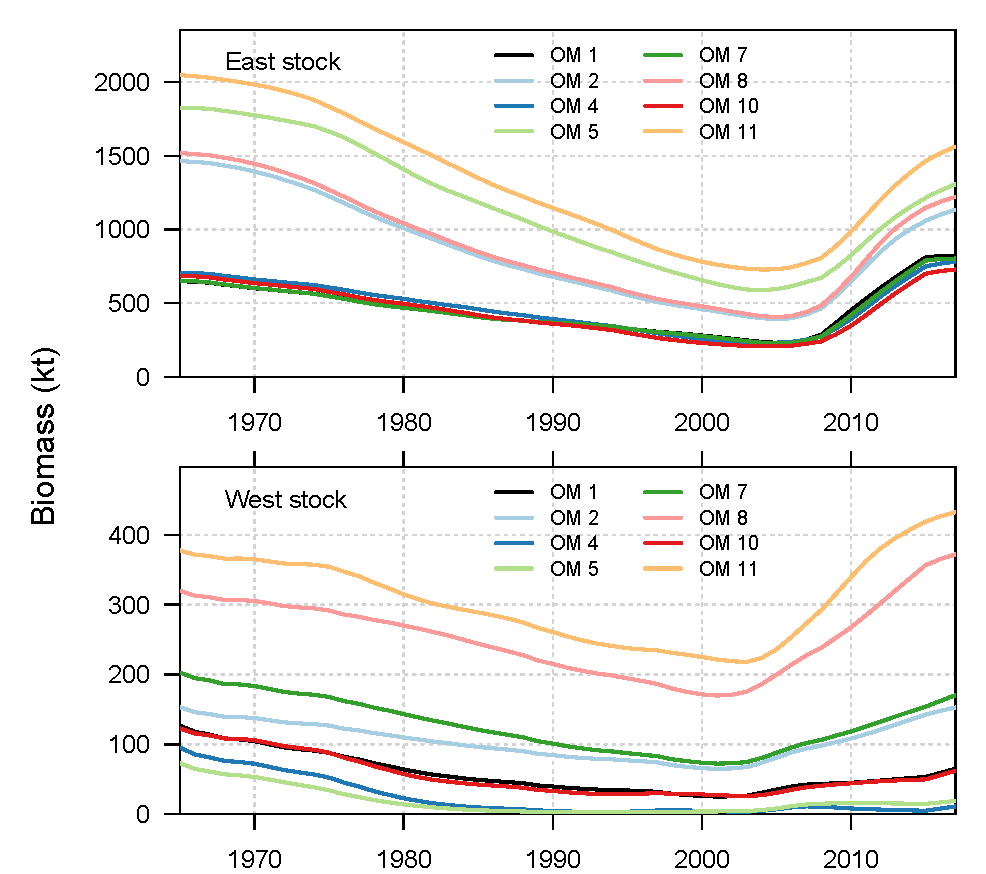
\includegraphics[width=0.9\linewidth]{data/OMbiomass} 

}

\caption{Operating model spawning stock biomasses for the full reference grid for both the Mediterannean stock (East) and Gulf of Mexico stock (West). Each colour corresponds to a different OM from the reference grid.}\label{fig:heatMapPlot}
\end{figure}

\begin{figure}[htb]

{\centering 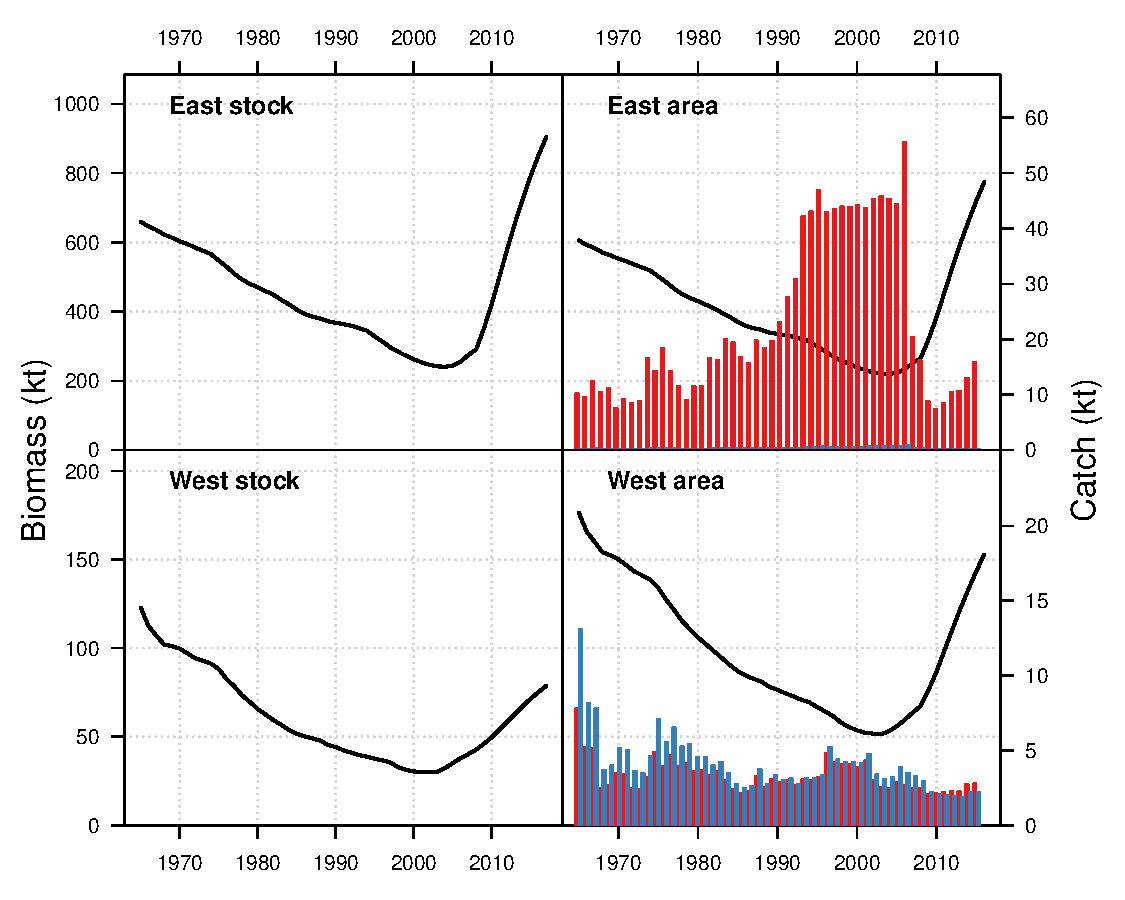
\includegraphics[width=0.9\linewidth]{data/AM/1/biomass} 

}

\caption{Spawning stock biomass estimates by stock (left hand column) and area (right hand column) from the delay difference stock assessment model fit to OM 1. Total area catch is shown split into East stock (red bars) and West stock (blue bars). Note that the catch scale is exaggerated with respect to the biomass, so that West stock catch is visible in the East area.}\label{fig:amBiomassPlot}
\end{figure}

\begin{figure}[htb]

{\centering 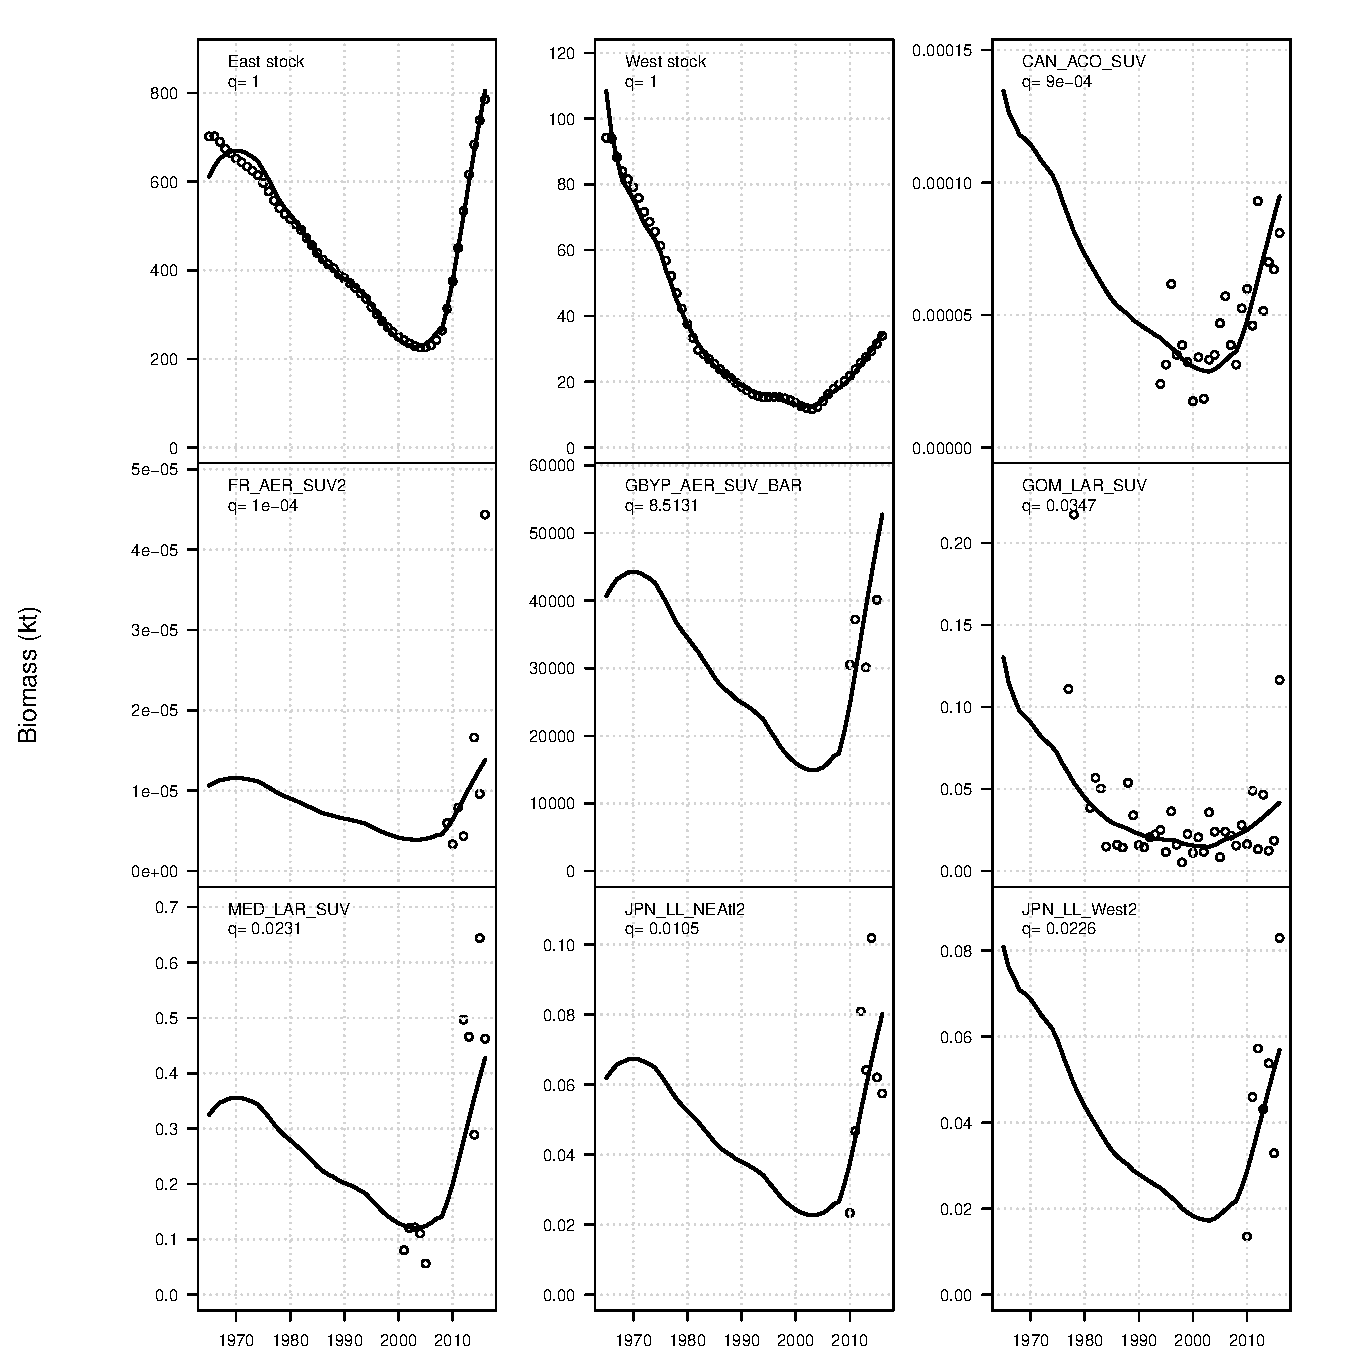
\includegraphics[width=0.9\linewidth]{data/AM/1/indexFits} 

}

\caption{Fits of the delay difference stock assessment model to stock and area management indices, with the associated catchability estimates. Data are shown as circles, while the lines indicate the model biomass scaled by catchability. East Stock and West Stock indices are the spawning stock biomass estimates from operating model 1.}\label{fig:amIdxFitsPlot}
\end{figure}

\begin{figure}[htb]

{\centering 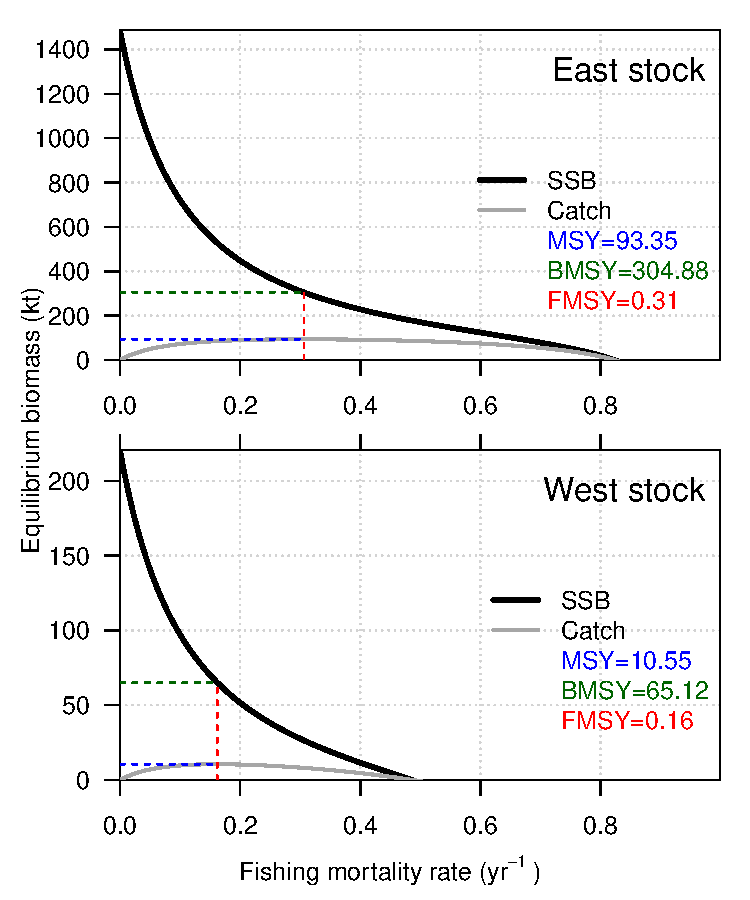
\includegraphics[width=0.9\linewidth]{data/AM/1/BRP} 

}

\caption{Equlibrium biomass (black) and yield (grey) curves as a function of fishing mortality estimated by the delay difference model fits to the management indices and operating model 1 spawning stock biomass.}\label{fig:amRefPtsPlot}
\end{figure}

% Add biblography
\newpage
\singlespacing 





\end{document}
